\documentclass[12pt,a4paper,eval,firamath]{nsi}
\pagestyle{empty}
\begin{document}
\titre{Machines de Turing }
\classe{NSI1}
\maketitle

\textbf{1.} Bien écouter la présentation de la machine de Turing par le professeur. Ne pas hésiter à poser des questions si certaines choses ne sont pas claires.\\


\textbf{2.} Insérer le \textbf{programme 1}  dans la machine. Pour chaque état initial :
\begin{itemize}
	\item recopier l'état sur le ruban \textbf{au crayon à papier};
    \item mettre la machine dans l'état 1;
    \item dérouler le programme en effaçant si besoin est les cases et en recopiant les nouveaux symboles;
    \item \textbf{s'il y a un état final}, l'indiquer sur cette copie en le recopiant et mettre une flèche en dessous de la case sur laquelle la machine s'arrête;
    \item \textbf{s'il n'y a pas d'état final}, indiquer ce qui se passe en commentaires.
    \item  Tu peux également utiliser les commentaires pour décrire globalement ce que fait le programme.
\end{itemize}
\begin{center}
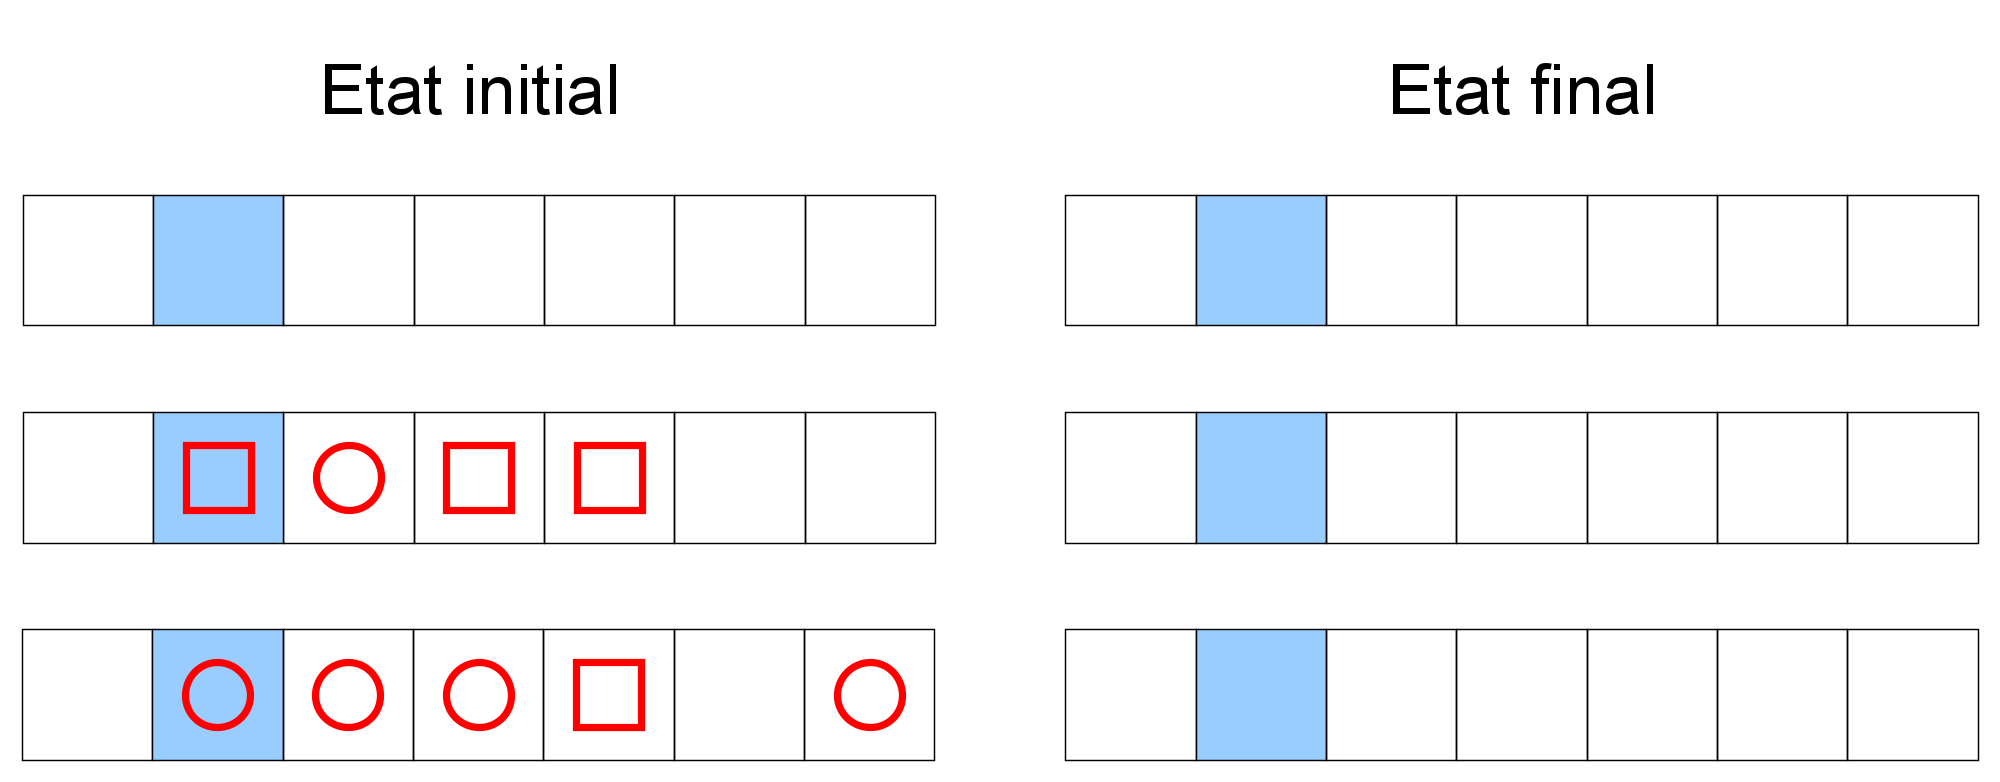
\includegraphics[width=17cm]{img/prog1}
\end{center}
\newpage
\textbf{Commentaires éventuels}\\

\carreauxseyes{16.8}{3.2}\\

\textbf{2.} Faire de même avec le \textbf{programme 2}.

\begin{center}
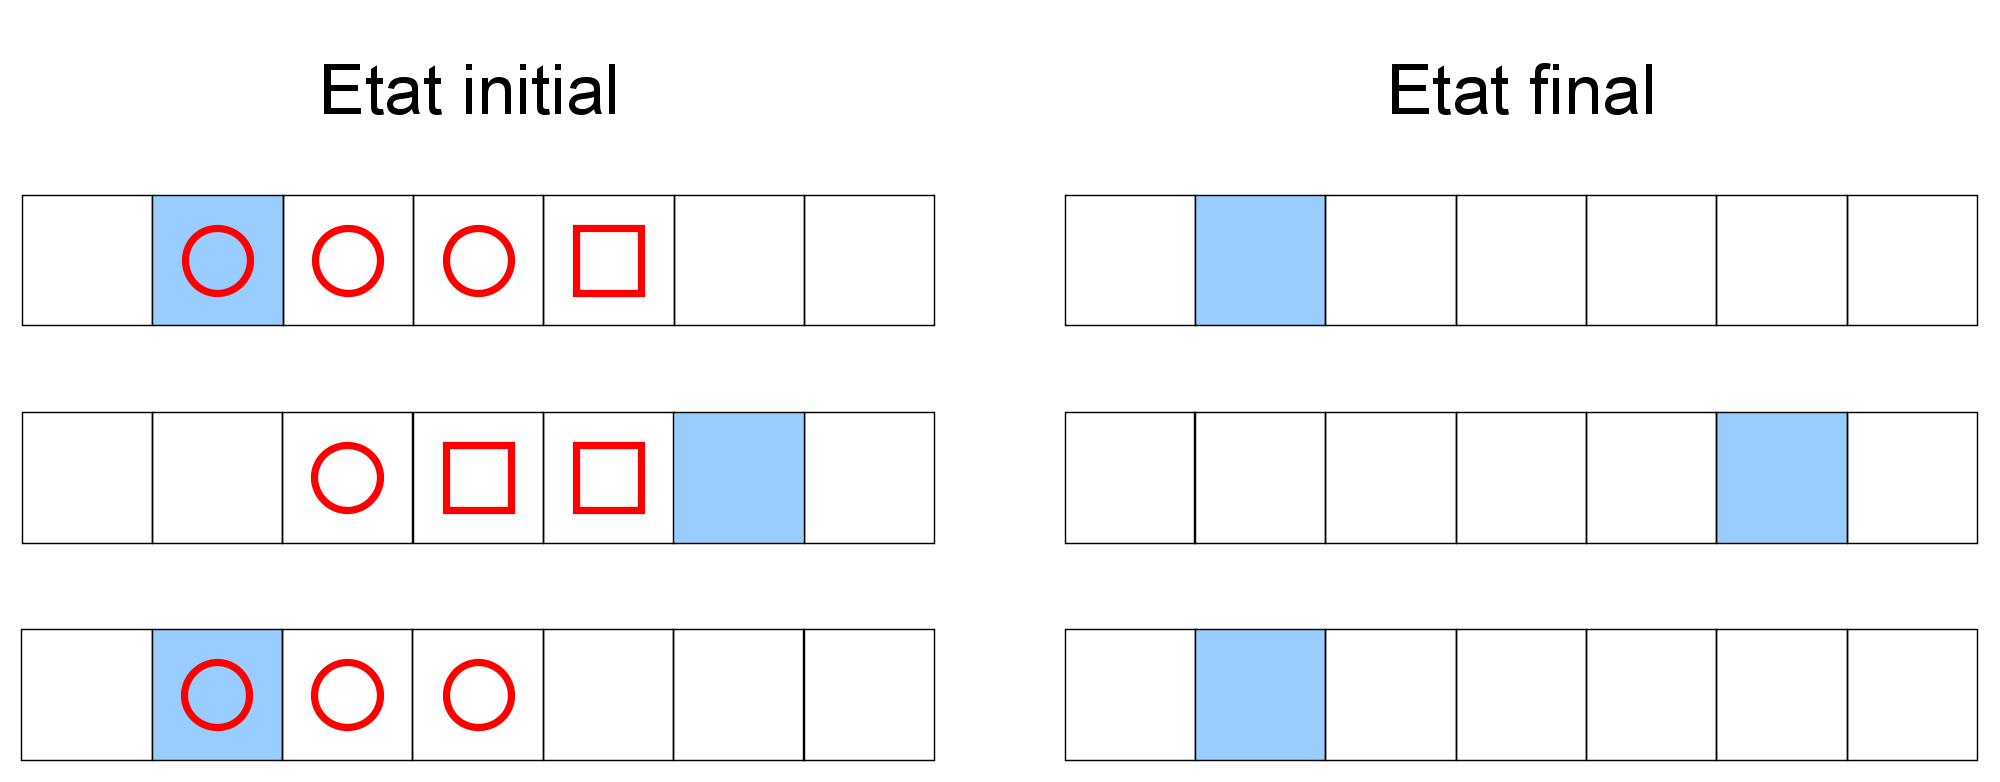
\includegraphics[width=17cm]{img/prog2}
\end{center}

\textbf{Commentaires éventuels}\\

\carreauxseyes{16.8}{4.8}\\

\textbf{3.} Le programme 3 est plus compliqué: les symboles sont des 0 et des 1 et ce que l'on représente sur le ruban, c'est l'écriture binaire d'un nombre.\\
\textbf{regarde d'abord la dernière page} pour comprendre son déroulement sur un exemple : tu peux faire comme l'exemple pas-à-pas.

Quelles sont les écritures décimales de $(100)_2$, $(110)_2$ et $(101)_2$ ?\\

\carreauxseyes{16.8}{6.4}\\




\begin{center}
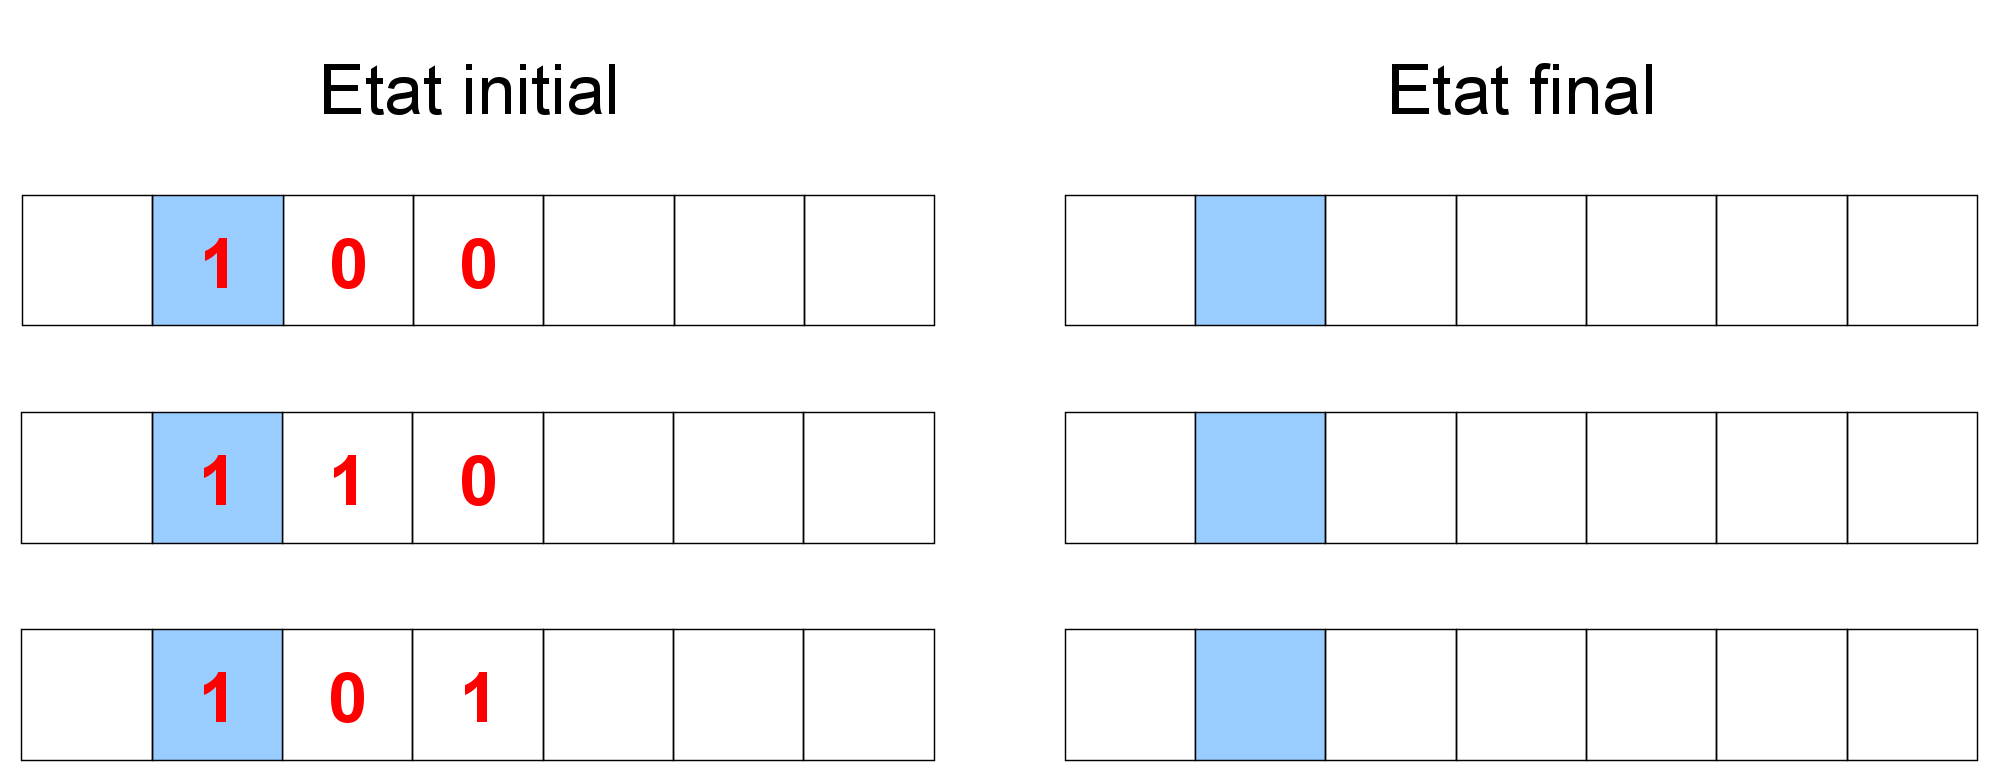
\includegraphics[width=17cm]{img/prog3}
\end{center}

\textbf{Commentaires éventuels}\\

\carreauxseyes{16.8}{8}

\newpage
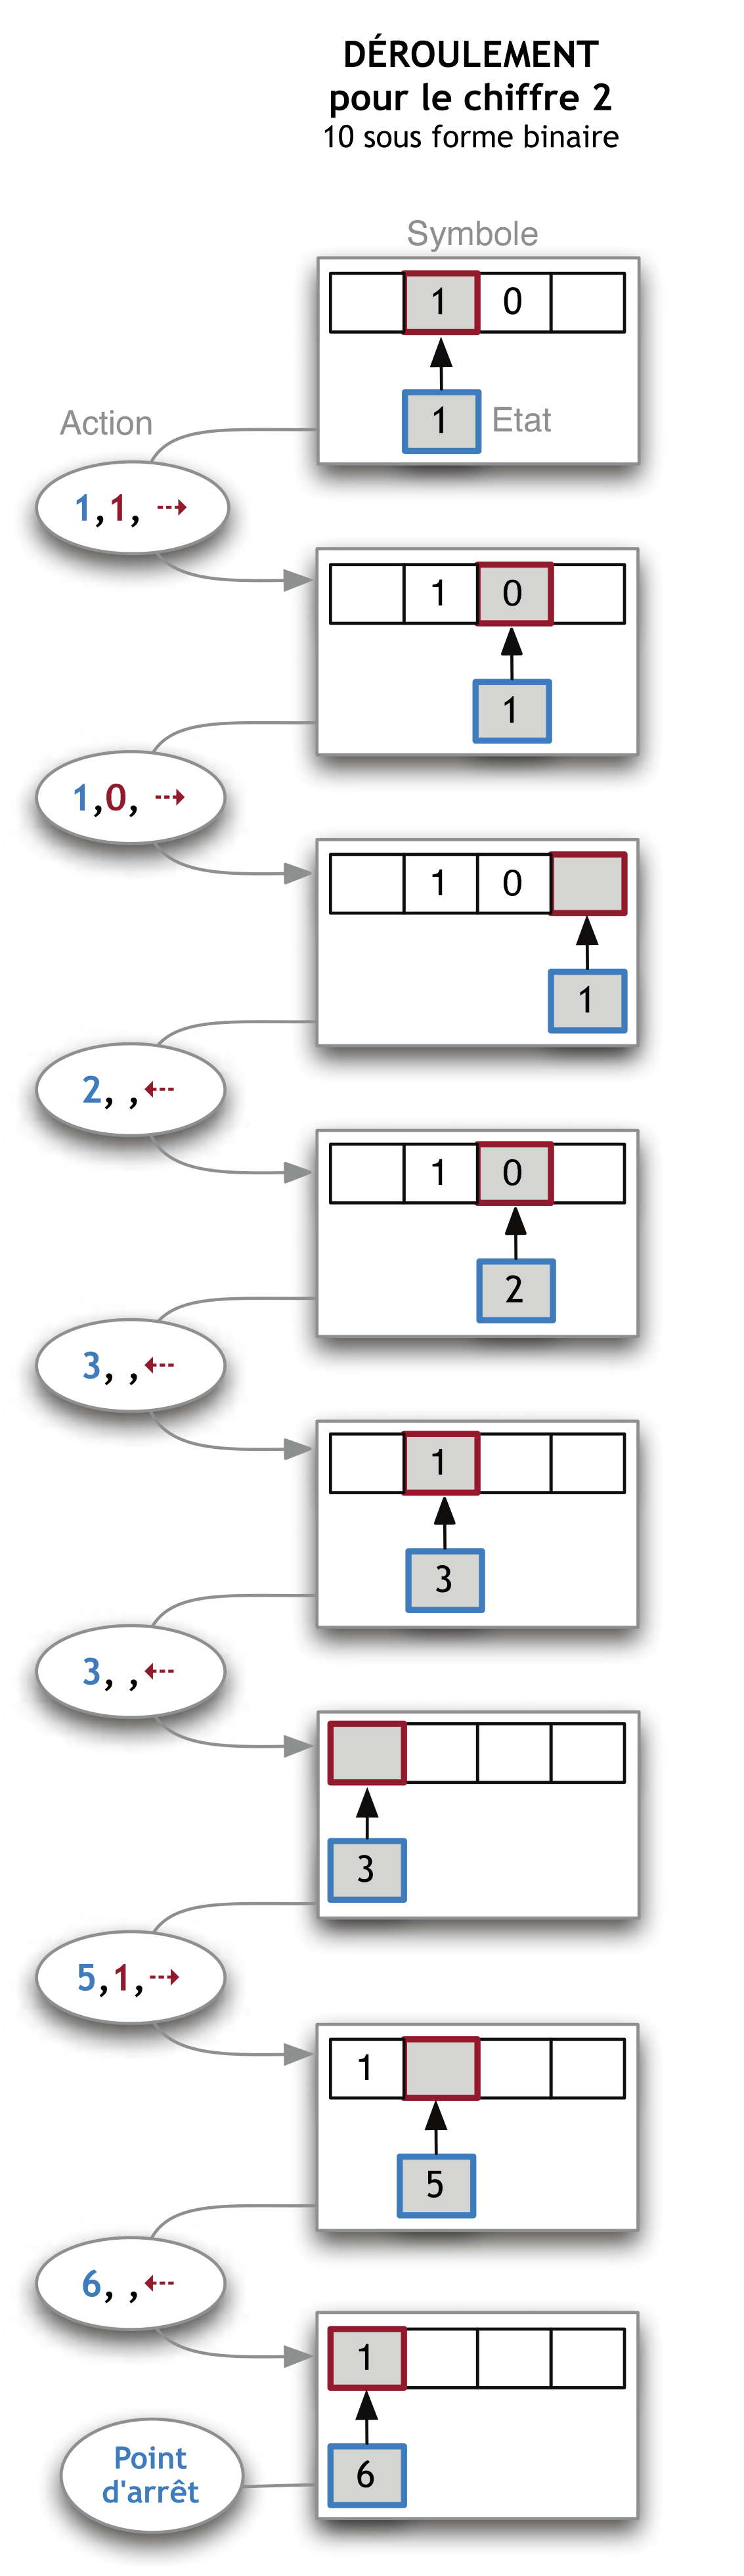
\includegraphics[height=25.7cm]{img/exprog3}
\end{document}